\newpage
\section{RS485}
    \subsection{Generelles}
        Ist ein Industriestandard der eine asynchrone serielle Datenübertragung ermöglicht. \\
        Der Standard verwendet ein symmetrisches Leitungspaar, dass für eine höhere elektromagnetische Resistenz sorgt.\\\\

    \subsection{Wie funktioniert es?}
        Betriebsspannung 5V oder 3.3V\\
        Der empfänger wertet die die Differenz beider Leitungen aus und kann Pegel ab $\pm 200mV$ erkennen.\\
        Senderpegel können von $\pm 1.5V bis \pm 6V$\\
        Logik: \\
        Wenn $U_{+} - U_{-} < -0.3V$ = MARK = OFF = Logisch 1\\
        Wenn $U_{+} - U_{-} > +0.3V$ = SPACE = ON = Logisch 0 \\


        \begin{figure}[!htb]
            \centering
            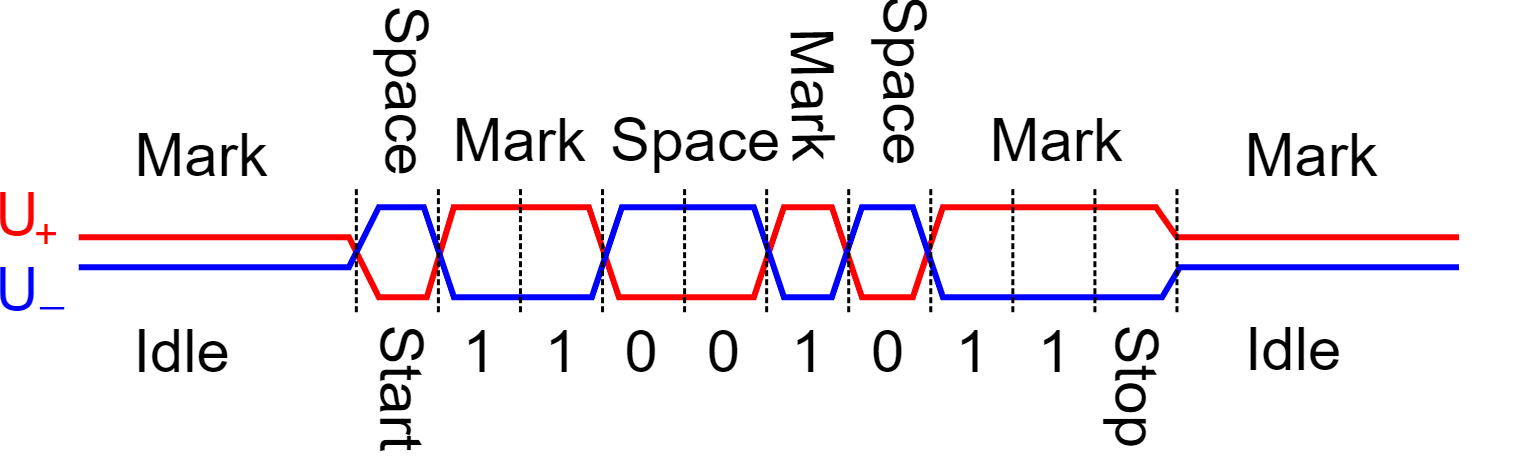
\includegraphics[scale=0.45]{RS485-Diagramm.png}
            \caption{RS485-Diagramm}
            \label{caption:RS485-Diagramm}
        \end{figure}
        

\newpage
    \subsection{Wie wird der MAX485 angeschlossen}
        
        Unten ist ein Beispiel mit einem Arduino UNO\\
        Anschluss:\\
        DI $\rightarrow$ TX\\
        RO $\rightarrow$ RX\\
        DE, RE auf einen GPIO Pin. Da wenn DE + RE = 1 $\rightarrow$ Daten können nur gesendet werden.\\
        Wenn DE + RE = 0 $\rightarrow$ Daten können nur empfangen werden.\\\\
    
        \begin{figure}[!htb]
            \centering
            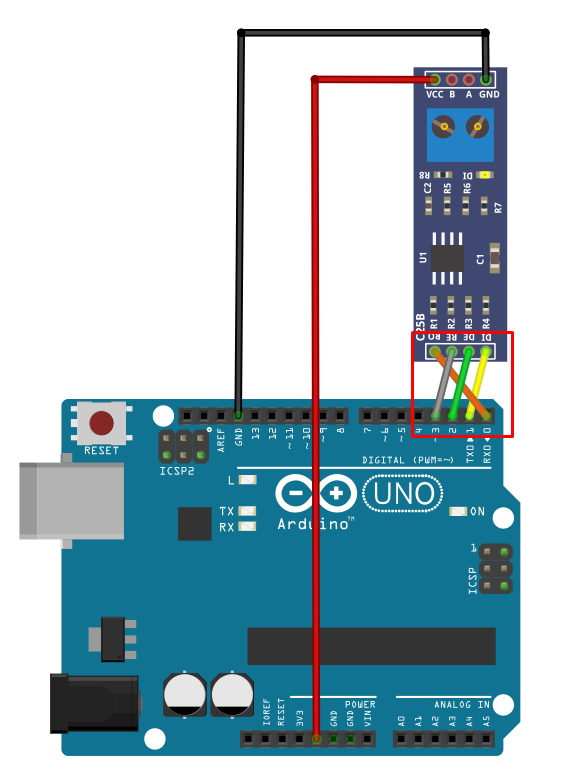
\includegraphics[scale=0.5]{MAX485-Arduino-Anschluss-BSP.png}
            \caption{MAX485-Arduino-Anschluss-BSP}
            \label{caption:MAX485-Arduino-Anschluss-BSP}
        \end{figure}

\newpage
        \noindent Ebenso muss dann der MAX485 and dem STM angeschlossen werden. Das untere Bild ist das Demo Board des STM32F030F4, eines der wenigen Boards, dass man zum Testen des Programmes 
        für den STM Chip kaufen kann.
    
        \begin{figure}[!htb]
            \centering
            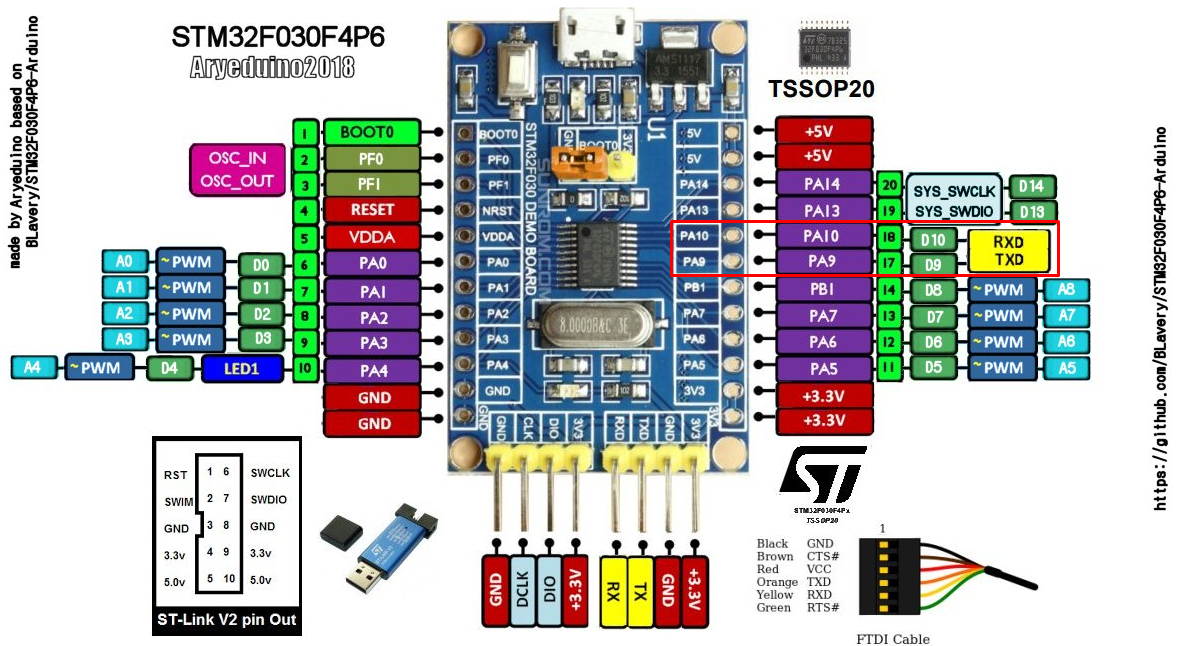
\includegraphics[scale=0.5]{STM32F030F4P6-Pinout.png}
            \caption{STM32F030F4P6-Pinout}
            \label{caption:STM32F030F4P6-Pinout}
        \end{figure} 
        